\section{Vercel}

El despliegue de la aplicación se realiza utilizando \textit{Vercel}, una plataforma de hosting orientada a aplicaciones frontend y serverless. La principal razón por la que se ha seleccionado esta plataforma, de entre las muchas opciones, es porque \textit{Vercel} es la empresa desarrolladora del framework \textit{Next.js}. Con esto se asegura una integración completa y se simplifica significativamente el proceso de despliegue.

También ha sido importante el hecho de que la infraestructura de \textit{Vercel} se apoya en servicios como \textit{Amazon Web Services} y \textit{Cloudflare} \cite{vercelInfrastructure2023}, entidades muy conocidas y confiadas, que proporcionan características de seguridad, disponibilidad y alto rendimiento. Sobre ellas, \textit{Vercel} ofrece una interfaz muy cómoda para manejar los despliegues, además de un sistema de despliegue continuo muy accesible.

\section{Límites y Características}

Para este proyecto, el plan gratuito \textbf{Hobby} de \textit{Vercel} ofrece unas características suficientes, ya que está dirigido a proyectos personales o de pequeña escala. En la tabla \ref{tab:vercel_plan_hobby}, se listan los principales límites de los recursos disponibles:

\begin{table}[htbp]
    \centering
    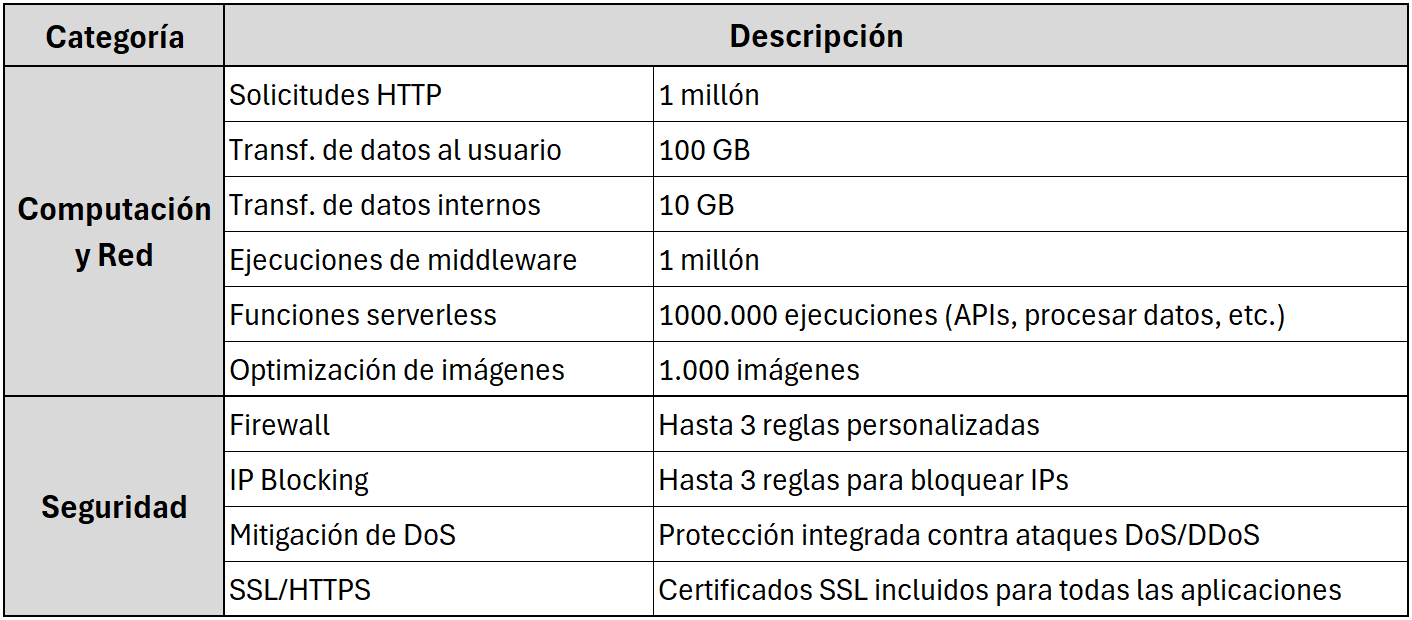
\includegraphics[width=0.9\textwidth]{figures/despliegue/vercel_plan_hobby.png}
    \captionsetup{skip=10pt}
    \caption{Límites y características por mes del plan \textit{Hobby} de \textit{Vercel}.}
    \label{tab:vercel_plan_hobby}
\end{table}

\section{Proceso de Despliegue}

El despliegue de la aplicación en \textit{Vercel} es muy sencillo, ya que la plataforma permite conectar un repositorio \textit{GitHub} para crear un nuevo proyecto y cargar todo el código. Además, al tratarse de un proyecto de \textit{Next.js}, la plataforma se encarga de establecer la configuración óptima para el build (figura \ref{fig:creacion_proyecto}).

\begin{figure}[H]
    \centering
    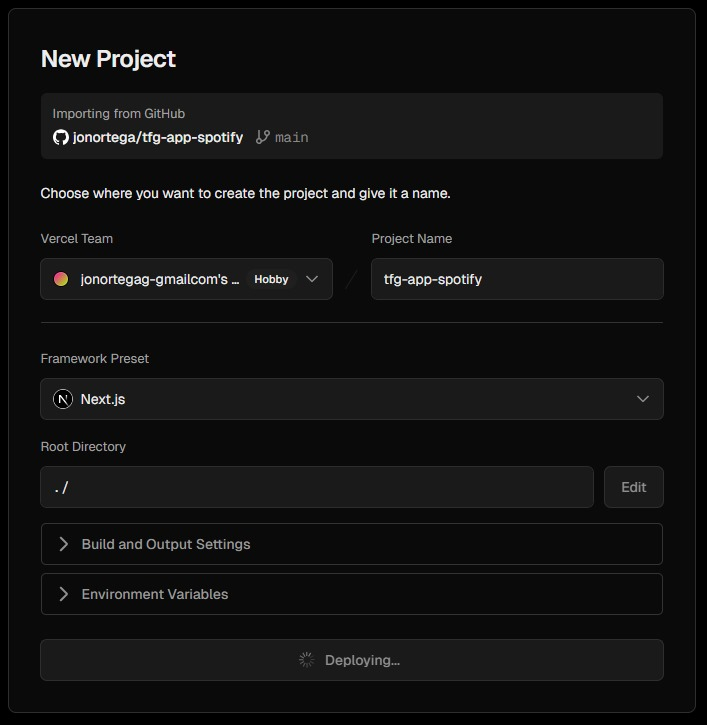
\includegraphics[width=0.5\textwidth]{figures/despliegue/creacion_proyecto.jpg}
    \caption{Pantalla de creación del proyecto tras conectarlo con el repositorio de \textit{GitHub}.}
    \label{fig:creacion_proyecto}
\end{figure}

Tras esperar a que se realice el buid correctamente, nuestra aplicación se encontrará en línea, con certificados SSL y con un dominio personal que \textit{Vercel} establecerá según el nombre del proyecto\footnote{Dominio del proyecto de este TFG: \href{https://tfg-app-spotify.vercel.app}{https://tfg-app-spotify.vercel.app}}. Existen dos diferentes entornos de despliegue:

\begin{itemize}
    \item \textit{Production}: Entorno principal, accesible para los usuarios finales desde el dominio establecido en la creación del proyecto. Se toma la rama \texttt{main} como la rama de producción.
    \item \textit{Preview}: Entorno de preproducción que se genera automáticamente al realizar cambios en cualquier rama distinta a la de producción (\texttt{main}). Se asigna un dominio único diferente a cada despliegue.
\end{itemize}

En nuestro caso, solo haremos uso del entorno \textit{production}. Cualquier cambio realizado en la rama \texttt{main} será detectado automáticamente por \textit{Vercel}, que creará un nuevo despliegue, realizará un nuevo build y actualizará la página en línea. En caso de que ocurra algún error, se revertirá automáticamente a la versión anterior del proyecto. Este proceso se realiza sin intervención manual, por lo que obtenemos un despliegue continuo (CD) sin necesidad de configuraciones adicionales.

\subsection{Configuración de Variables de Entorno}

Para finalizar con la configuración del despliegue, es necesario agregar las variables de entorno en el panel de control de \textit{Vercel}. Cada entorno permite establecer variables específicas, pero en nuestro caso solo introduciremos, en el entorno de producción, las siguientes:

\begin{table}[htbp]
    \centering
    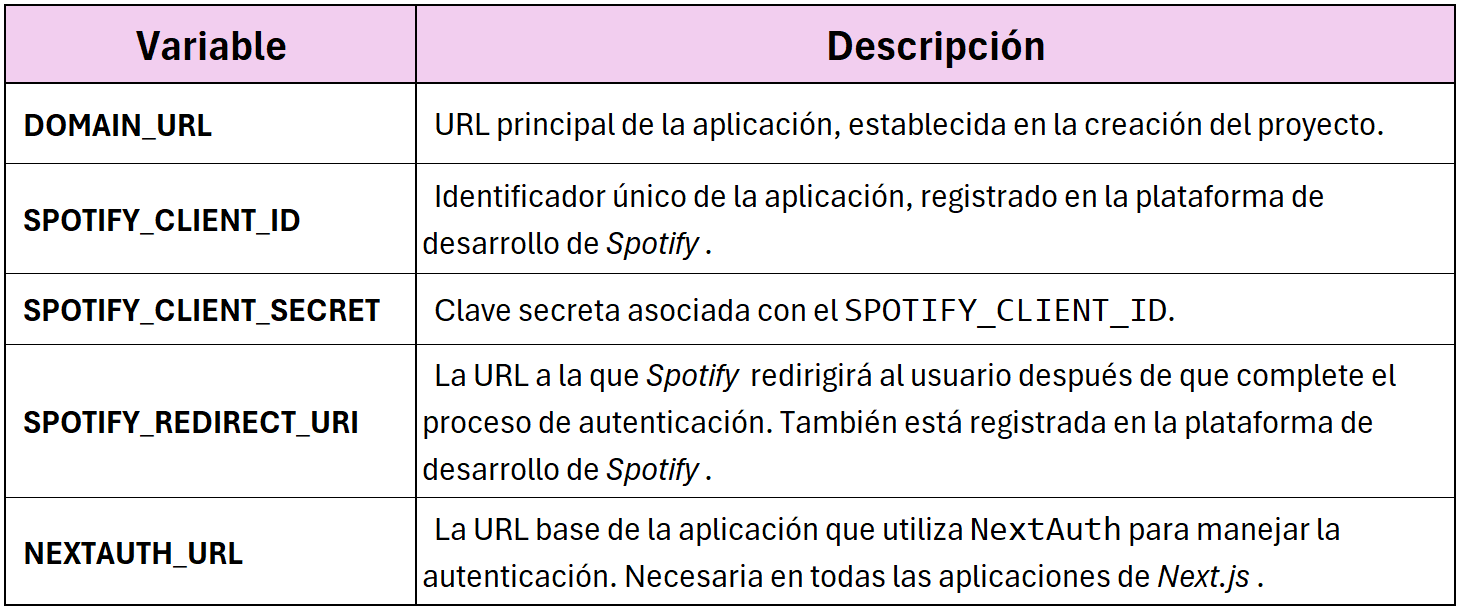
\includegraphics[width=0.9\textwidth]{figures/despliegue/variables_entorno.png}
    \captionsetup{skip=10pt}
    \caption{Variables de entorno necesarias en producción.}
    \label{tab:variables_entorno}
\end{table}

Es importante destacar que, para garantizar una transición fluida entre el entorno de desarrollo local y el de producción, se debe evitar codificar directamente las URLs en el código. En su lugar, se debe utilizar la variable de entorno \texttt{DOMAIN\_URL}, lo que permite que las URLs cambien automáticamente de \texttt{localhost} al dominio público correspondiente.

\subsection{Análisis y Monitoreo}

\textit{Vercel} ofrece un panel de control desde donde se pueden visualizar diversas métricas y modificar opciones de configuración. Es importante monitorizar los indicadores de recursos consumidos (figura \ref{fig:usage_overview}), para asegurar que no llegan al límite del plan gratuito.

\begin{figure}[H]
    \centering
    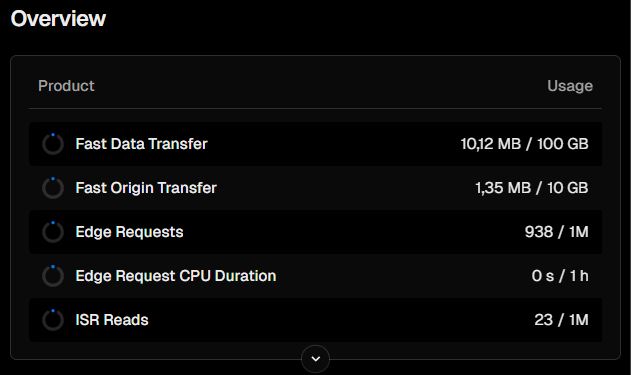
\includegraphics[width=0.6\textwidth]{figures/despliegue/usage_overview.png}
    \caption{Panel con la visión general de los recursos consumidos.}
    \label{fig:usage_overview}
\end{figure}

\newpage

Esto es especialmente relevante porque, en las plataformas de nube, se ha popularizado un ataque conocido como \textbf{Ataque de Agotamiento Económico} (\textit{Denial of Wallet} (DoW)) \cite{vercelDoW2025}. Son un tipo de ataque DoS, cuyo objetivo es consumir continuamente los recursos más ``pesados'', con el fin de obligar el escalado automático y agotar el presupuesto operativo de la aplicación. En el caso de este proyecto, al encontrarse dentro del plan gratuito, la consecuencia sería el consumo completo de los recursos disponibles; haciendo que \textit{Vercel} retirase la aplicación de producción, quedándose inoperativa hasta el siguiente ciclo mensual.

Por esta razón, \textit{Vercel} y otras plataformas similares ofrecen mecanismos de protección contra ataques DoS, permitiendo bloquear temporalmente este tipo de peticiones con el firewall integrado. Además, podemos acceder a ver los logs generados en el servidor durante la última hora y monitorizar el número de invocaciones, datos transferidos y peticiones por cada ruta de nuestra web.

\section{Ejecución Automática de Tests} \label{sec:test_automaticos}

Para poder realizar la ejecución de los tests de manera automática, se debe crear un fichero de workflow dentro de la ruta \texttt{.github/workflows/} en la raíz del proyecto. En este caso, se ha creado un fichero \textbf{\texttt{test-and-deploy.yml}} (fichero en \hyperref[ch:anexoF]{Anexo F}). Dentro de éste, se establecen los pasos que \textit{GitHub Actions} debe realizar para la configuración del entorno, la ejecución de las pruebas y el despliegue.

Este workflow consta de dos jobs principales: el job de \textbf{pruebas} y el job de \textbf{despliegue}. Una de las particularidades más relevantes de esta configuración es que, debido a problemas con la dependencia \texttt{canvas}, se ha tenido que optar por un enfoque híbrido en la gestión de paquetes: se usa \textbf{npm para las pruebas} y \textbf{pnpm para el despliegue}. Esta decisión fue necesaria para evitar conflictos con las dependencias de \texttt{jest-environment-jsdom} y \texttt{canvas}, que generaban errores en la instalación cuando se intentaba usar \texttt{pnpm} en los tests. Adicionalmente, para garantizar que \texttt{pnpm} no genere problemas con la caché en el despliegue, se ha \textbf{desactivado la caché de pnpm} en el workflow.

\subsection*{Job de Pruebas}

El primer job, llamado \texttt{test}, se ejecuta en \texttt{ubuntu-latest} y está configurado para ejecutarse en cada \texttt{push} a las ramas \texttt{main} y \texttt{testing}. Este job comienza con la instalación de las dependencias necesarias para la compilación de \texttt{canvas}, ya que esta librería requiere la instalación de paquetes del sistema operativo. A continuación, se instala \texttt{Node.js} y se ejecuta la instalación de dependencias con \texttt{npm}, utilizando la opción \texttt{--legacy-peer-deps}, muy importante para evitar errores de resolución de dependencias entre \texttt{canvas} y \texttt{jest-environment-jsdom}.

Tras la instalación de dependencias, se realiza un rebuild de \texttt{canvas} para asegurar su correcta compilación en el entorno de ejecución. Luego, se procede a la compilación del proyecto con \texttt{npm run build} y, finalmente, se ejecutan los tests con \texttt{npm test}. \textbf{En caso de que los tests fallen, el proceso se detiene y no se ejecuta el despliegue}.

\subsection*{Job de Despliegue}

Si el job de pruebas finaliza correctamente, se ejecuta el job de \texttt{deploy}, el cual se encarga de desplegar la aplicación en \textit{Vercel}. Para ello, primero se realiza un nuevo \texttt{checkout} del repositorio y se instala \texttt{Node.js} en la misma versión utilizada en los tests. Dado que el proyecto ha sido desarrollado con \texttt{pnpm}, en este punto se instala \texttt{pnpm}.

Posteriormente, se instalan las dependencias con \texttt{pnpm install --frozen-lockfile} para garantizar que sea consistente con el archivo \texttt{pnpm-lock.yaml}. A continuación, se instala la CLI de \texttt{Vercel} utilizando \texttt{pnpm dlx vercel@latest pull}, lo que permite obtener la configuración de despliegue de la aplicación. Finalmente, \textbf{se ejecuta el despliegue en producción mediante \texttt{pnpm dlx vercel --prod}}.

\subsection{Configuración de Variables de Entorno}

Para que la aplicación y los tests funcionen correctamente en \textit{GitHub Actions}, es necesario configurar las variables de entorno en el repositorio. Estas variables incluyen las mismas credenciales que las configuradas para el despliegue en \textit{Vercel} y se deben configurar en el repositorio \textit{GitHub}.

Además, se debe añadir el \textbf{token de Vercel} para permitir el despliegue automático de la aplicación. Para ello, se debe generar un nuevo token en la configuración de \textit{Vercel} y añadirlo en los \texttt{Secrets} del repositorio con el nombre \texttt{VERCEL\_TOKEN}. Esto permitirá que \textit{GitHub Actions} pueda autenticar y desplegar la aplicación en producción sin intervención manual.

\subsection{Flujo CI/CD Final}

Con la configuración establecida en este workflow, cualquier \textbf{push} a la rama \texttt{main} en \textit{GitHub} activará automáticamente el proceso de ejecución de tests y, si estos pasan correctamente, se procederá con el despliegue en \textit{Vercel}. Este flujo garantiza que cualquier cambio en la aplicación se valide antes de ser publicado en producción.

Para visualizar la correcta ejecución del proceso, se han capturado dos imágenes donde se puede observar que el mismo commit aparece tanto en la sección de \textit{GitHub Actions}, donde se registran los tests y el despliegue, como en el entorno de producción de \textit{Vercel}, confirmando así que los cambios han sido desplegados exitosamente.

\begin{figure}[H]
    \centering
    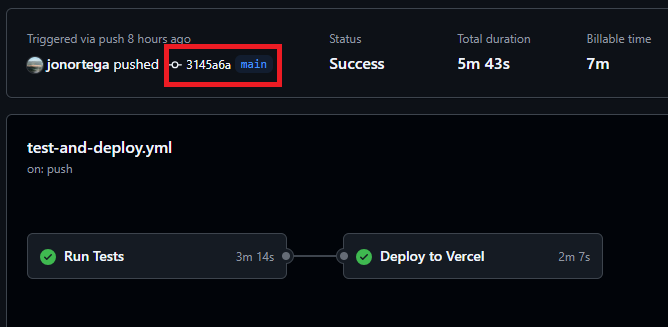
\includegraphics[width=0.75\textwidth]{figures/despliegue/github_actions.png}
    \caption{Workflow en \textit{GitHub Actions}: ejecución de tests y despliegue en \textit{Vercel} tras un push a \texttt{main}.}
    \label{fig:github_actions}
\end{figure}

\begin{figure}[H]
    \centering
    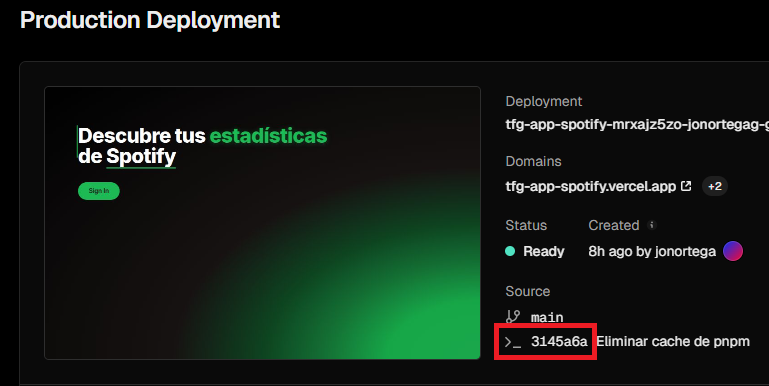
\includegraphics[width=0.75\textwidth]{figures/despliegue/actions_deploy_vercel.png}
    \caption{Despliegue exitoso en \textit{Vercel} con el mismo commit de \textit{GitHub Actions}.}
    \label{fig:actions_deploy_vercel}
\end{figure}